% !TeX root = main.tex
\section*{Lithographic system}
The basic working of contact lithography is illustrated in figure \ref{fig:contact-litho}. Light emitted from a source is collimated using a condenser lens (or an array of lenses). The collimated light travels through the transparent parts of the mask and illuminates the resist areas directly below these areas. 
\begin{figure}[H]
	\centering
	\resizebox{0.7\linewidth}{!}{% !TeX root = main.tex
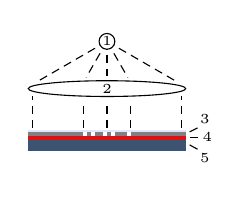
\begin{tikzpicture}
    % Sample
    \fill[fill={rgb:red,66;green,91;blue,121}] (-1,-1.24) rectangle (1,-1.39);
    \draw (1.05,-1.315) to node [below right = -.4 mm] {\tiny $5$} (1.15,-1.37);
    % Resist
    \fill[fill={rgb:red,198;green,15;blue,15}] (-1,-1.20) rectangle (1,-1.24);
    \draw (1.05,-1.22) to node [right = -.1 mm] {\tiny $4$} (1.15,-1.22);
    % Mask
    \foreach \x/\y in {0/.7,.75/.8,.85/0.95,1/1.05,1.1/1.25,1.3/2}
        \fill[fill=gray] (\x-1,-1.15) rectangle (\y-1,-1.20);
    \draw (1.05,-1.15) to node [above right = -.4 mm] {\tiny $3$} (1.15,-1.10);
    % Glass plate
    \fill[fill=blue!10] (-1,-1.12) rectangle (1,-1.15);
    % Lens
    \draw (0,-.6) ellipse [x radius=1, y radius=.1] node {\tiny $2$};
    % Light rays
    \foreach \angle/\r in {210/1,240/.53,270/.44,300/.53,330/1}
        \draw[densely dashed] (0,0) -- (\angle:\r);
    \foreach \x/\y in {-.95/.7,-.3/.75,0/.75,.3/.75,.95/.7}
        \draw[densely dashed] (\x,-1.1) -- (\x,-\y);
    % Light source
    \draw[fill=white] (0,0) ellipse [x radius=.1, y radius=.1] node {\tiny $1$};
\end{tikzpicture}
}
	\caption{Simplified working of contact lithography, where 1. light source, 2. condenser lens(es), 3. glass plate with mask, 4. photographic resist, 5. substrate. Dashed lines indicate light paths.}
	\label{fig:contact-litho}
\end{figure} A MJB-3 from Karl Suss Microtec was used with a modification. 

A mask was created, with both the original design and an inverted version. \todo[inline]{ meer info} 

\section*{Substrate and resist}
A series of square cut silicon substrates of approximately 15 mm by 15 mm were used. Resist consists of \todo[inline]{kenneth's stukje}

\begin{figure}[H]
	\centering
	\begin{subfigure}[t]{0.45\linewidth}
		\centering
		\resizebox{\linewidth}{!}{% !TeX root = main.tex
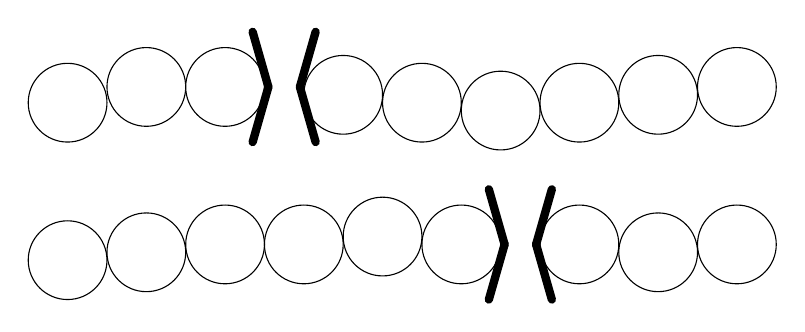
\begin{tikzpicture}
    % Polymer beads
    \foreach \x/\y in {0/0,1/.1,2/.2,3/.2,4/.3,5/.2,6.5/.2,7.5/.1,8.5/.2}
        \draw (\x,\y) circle (5mm);
    % Polymer beads
    \foreach \x/\y in {0/0,1/.2,2/.2,3.5/.1,4.5/0,5.5/-.1,6.5/.0,7.5/.1,8.5/.2}
        \draw[black,fill=white] (\x,2+\y) circle (5mm);
    % Scissors
    \begin{scope}[line width=3,line cap=round]
        % Left scissor
        \draw (5.55,.2) -- (5.35,.9);
        \draw (5.55,.2) -- (5.35,-.5);
        % Right scissor
        \draw (5.95,.2) -- (6.15,.9);
        \draw (5.95,.2) -- (6.15,-.5);
        
        % Left scissor
        \draw (2.55,2.2) -- (2.35,2.9);
        \draw (2.55,2.2) -- (2.35,1.5);
        % Right scissor
        \draw (2.95,2.2) -- (3.15,2.9);
        \draw (2.95,2.2) -- (3.15,1.5);
    \end{scope}
\end{tikzpicture}
}
		\caption{Chain scissors}
		\label{fig:chainscissor}
	\end{subfigure}
	~
	\begin{subfigure}[t]{0.45\linewidth}
		\centering
		\resizebox{\linewidth}{!}{% !TeX root = main.tex
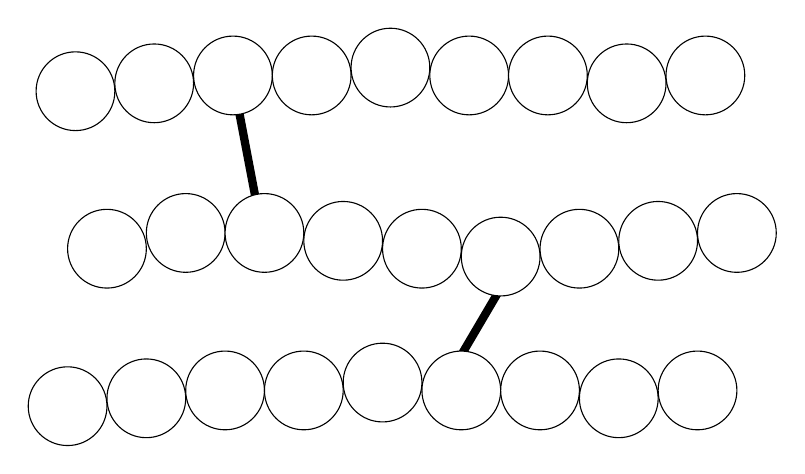
\begin{tikzpicture}
    % Cross links
    \begin{scope}[line width=3]
        \draw (5,.65) -- (5.5,1.5);
        \draw (2.5,2.05) -- (2.1,4.15);
    \end{scope}
    % Polymer beads
    \foreach \x/\y in {0/0,1/.1,2/.2,3/.2,4/.3,5/.2,6/.2,7/.1,8/.2}
        \draw[black,fill=white] (\x,\y) circle (5mm);
    % Polymer beads
    \foreach \x/\y in {0/0,1/.2,2/.2,3/.1,4/0,5/-.1,6/.0,7/.1,8/.2}
        \draw[black,fill=white] (.5+\x,2+\y) circle (5mm);
    % Polymer beads
    \foreach \x/\y in {0/0,1/.1,2/.2,3/.2,4/.3,5/.2,6/.2,7/.1,8/.2}
        \draw[black,fill=white] (.1+\x,4+\y) circle (5mm);
\end{tikzpicture}
}
		\caption{Cross-linking}
		\label{fig:crosslinking}
	\end{subfigure}
	\caption{Polymer changes}
	\label{fig:polymers}
\end{figure}

\todo[inline]{polymer chain images}

\section*{Recipe}
The used recipes for both the positive and negative resists are explained here.
\subsection*{Positive resist}
As a positive tone resist, AZ5214\footnote{Produced by MicroChemicals} is used. To promote adhesion to the Si substrate, HMDS (hexamethyldisilazane) is applied first as a primer. The primer is deposited by hand on top of a silicon wafer and spun at 4000 RPM, it is then baked on a hot plate at 200$^{\circ}$~C for two minutes. The resist is spun at the same speed as the primer, which should result in a layer thickness of $1.40 \mu$m. The resist is baked on a hot plate at 90$^{\circ}$~C for one minute.

When the resist is deposited, the sample is then exposed in a mask aligner for 2,3,4,5,6 and 8 minutes. After exposure the sample is developed for 60 seconds in MF321 and then development is stopped by rinsing the sample another 60 seconds in purified water.

\subsection*{Negative resist}
For the negative resist samples, the same AZ5241 is used, but with a slightly different recipe to make it negative tone. Up to the exposure, the negative resist recipe is the same as that for the positive tone. AZ5241 contains a special crosslinking agent which becomes active at temperatures above 110$^{\circ}$~C where the resist has been exposed. The crosslinking agent causes the individual molecules to bond, creating an almost insoluble, non-photoreactive substance. This allows the AZ5241 to also be used as a negative resist.

Using the same mask as for the positive exposure, the sample is illuminated for a period 1 \todo[inline]{check time} minutes. After this first illumination the sample is baked in an oven at ... \todo[inline]{temp?} $^\circ$~C for 45 seconds. During this time cross-links are formed in the resist that was exposed during the first illumination. During baking the sample lies on an aluminium slab inside the oven, this prevents a large decrease in temperature when the oven door is opened and ensures good heat transfer to the sample. After baking, the entire sample is exposed (flood exposure) for a period of either 1,2,3,4 \todo[inline]{all times} minutes. During this time the polymer chains in the areas of the resist that were not exposed during the first illumination, are cut up into smaller chains. In the next step, the development, these smaller chains are dissolved in the development solution \todo[inline]{name}. After development, the sample is rinsed with purified water as was done with the positive resist samples.